\documentclass[conference]{IEEEtran}
\IEEEoverridecommandlockouts
% The preceding line is only needed to identify funding in the first footnote. If that is unneeded, please comment it out.
\usepackage{cite}
\usepackage{amsmath,amssymb,amsfonts}
\usepackage{algorithmic}
\usepackage{graphicx}
\usepackage{textcomp}
\usepackage{xcolor}
\usepackage{float} % Add the float package for H specifier
\def\BibTeX{{\rm B\kern-.05em{\sc i\kern-.025em b}\kern-.08em
    T\kern-.1667em\lower.7ex\hbox{E}\kern-.125emX}}
\usepackage{listings}
\lstset{
basicstyle=\small\ttfamily,
columns=flexible,
breaklines=true
}
\begin{document}
\onecolumn
\title{CSC 693 - HW 1 - LDA}
\author{Sahil Dhawan}
\maketitle
\section{Text Preprocessing}
\begin{enumerate}
    \item Split comments into sentences and report the average number of sentences per comment.\\
    \hspace{1cm}Average number of setences per comment = 10.704\\
    \item Do tokenization for the dataset and report the average number of tokens per comment.\\
    \hspace{1cm}Average number of words per comment = 146.841\\
    \item Without considering punctuation and stop words, how many words are in each comment on average?\\
    \hspace{1cm}Average number of words per comment, excluding stop words and punctuation = 99.654\\
    \item Try lemmatization and stemming for the database. What are the differences in the results based on your observation?\\
    \hspace{1cm}Average number of words per comment:
    \begin{itemize}
        \item Lemmatization\\
        \hspace{1cm}including stop words and punctuation: 144.087\\
        \hspace{1cm}excluding stop words and punctuation: 97.765
        \item Stemming\\
        \hspace{1cm}including stop words and punctuation: 142.546\\
        \hspace{1cm}excluding stop words and punctuation: 95.841
    \end{itemize}
    Lemmatization and Stemming create an almost equal amount of average words per comment, both including and excluding stop words and punctuation. The text file from the 50th index of parsed file names shows a sample data comparison between the original file and lemmatization and stemming of the file (excluding stop words and punctuation).\\
    Original "145\_10.txt":
    \begin{lstlisting}
Sequel to "The Kingdom" is bloodier and even more twisted. I only saw half (I was exhausted and couldn't sit through all 5 1/2 hours) but I loved what I saw. Ghosts, blood, murder, poisoning, mutated babies, voodoo...this has it all! If you have a strong stomach and like weird movies this is for you.<br /><br />Also, you don't have to see Part 1 to understand this...you'll figure it out!<br /><br />Does anyone know if Kingdom 1 and 2 are available on DVD? Sitting through these marathon movies in a theatre is tiring. <br /><br />Sadly, there probably won't be a "Kingdom 3"--Ernst-Hugo Jaregard (Sig) died a year after this was filmed. But you never know!
    \end{lstlisting}
    Lemmatization of "145\_10.txt":
    \begin{lstlisting}
['sequel', 'kingdom', 'bloodier', 'even', 'twisted', 'saw', 'half', 'exhausted', 'could', 'sit', '5', '1/2', 'hour', 'loved', 'saw', 'ghost', 'blood', 'murder', 'poisoning', 'mutated', 'baby', 'voodoo', 'strong', 'stomach', 'like', 'weird', 'movie', 'you.', 'also', 'see', 'part', '1', 'understand', 'figure', 'anyone', 'know', 'kingdom', '1', '2', 'available', 'dvd', 'sitting', 'marathon', 'movie', 'theatre', 'tiring', 'sadly', 'probably', 'wo', 'kingdom', '3', '--', 'ernst-hugo', 'jaregard', 'sig', 'died', 'year', 'filmed', 'never', 'know']
    \end{lstlisting}
    Stemming of "145\_10.txt":
	\begin{lstlisting}
['sequel', 'kingdom', 'bloodier', 'even', 'twist', 'saw', 'half', 'exhaust', 'could', 'sit', '5', '1/2', 'hour', 'love', 'saw', 'ghost', 'blood', 'murder', 'poison', 'mutat', 'babi', 'voodoo', 'strong', 'stomach', 'like', 'weird', 'movi', 'you.', 'also', 'see', 'part', '1', 'understand', 'figur', 'anyon', 'know', 'kingdom', '1', '2', 'avail', 'dvd', 'sit', 'marathon', 'movi', 'theatr', 'tire', 'sadli', 'probabl', 'wo', 'kingdom', '3', '--', 'ernst-hugo', 'jaregard', 'sig', 'die', 'year', 'film', 'never', 'know']
	\end{lstlisting}
Lemmatization reduces some words to a lemma form, such as "movies" to "movie", but keeps others the same such as "sitting". Stemming (PorterStemmer) reduces more words to their base form, such as "available" to "avail". Stemming may be more effective for LDA as different variations of a main topic word could be reduced to the same base form and show up easier in a frequency distribution.
\end{enumerate}
\newpage
\section{Topic Modeling}
\begin{enumerate}
    \item Use the Latent Dirichlet Allocation (LDA) method to discover latent topics in the dataset. Try different numbers of topics for LDA. What number of topics do you think is more meaningful?\\
    LDA with a dataset that included stop words and punctuation consistently showed tokens such as "the", ",", ".", "a", etc. to be the most likely topics, so only data that excludes tokens like these were processed with LDA. Lemmatization and Stemming produced the following with three topics:
\begin{lstlisting}
---3 Topics, Exclusion Lemmatization

Performing Latent Drichlet Allocation (3 topics)...
(0, '0.015*"film" + 0.010*"movie" + 0.008*"one" + 0.006*"like" + 0.005*"see" + 0.005*"story" + 0.004*"good" + 0.004*"character" + 0.004*"well" + 0.004*"show"')
(1, '0.013*"film" + 0.006*"time" + 0.006*"one" + 0.005*"movie" + 0.005*"like" + 0.004*"scene" + 0.004*"would" + 0.004*"story" + 0.003*"see" + 0.003*"make"')
(2, '0.019*"movie" + 0.013*"film" + 0.010*"one" + 0.005*"good" + 0.005*"character" + 0.005*"story" + 0.005*"great" + 0.005*"like" + 0.005*"time" + 0.004*"even"')
---3 Topics, Exclusion Stemming

Performing Latent Drichlet Allocation (3 topics)...
(0, '0.015*"movi" + 0.015*"film" + 0.010*"one" + 0.006*"stori" + 0.005*"like" + 0.005*"watch" + 0.005*"see" + 0.004*"time" + 0.004*"love" + 0.004*"make"')
(1, '0.016*"movi" + 0.015*"film" + 0.008*"one" + 0.007*"like" + 0.007*"good" + 0.006*"time" + 0.005*"see" + 0.005*"charact" + 0.005*"great" + 0.004*"well"')
(2, '0.014*"film" + 0.008*"movi" + 0.007*"like" + 0.007*"one" + 0.006*"love" + 0.005*"charact" + 0.005*"time" + 0.004*"see" + 0.004*"good" + 0.004*"great"')
\end{lstlisting}
The content of these topics are very similar, in terms of the string determined to be a topic or the synonyms of which string is a topic: for example, "film" and "movie" are the most likely topics but have the same meaning. Although the probablity distributions differ, it seems choosing 1 topic might be the most meanigngful and least redundant.\\
    \item Apply necessary text preprocessing techniques for the dataset. Are the topic modeling results better?\\
    As mentioned in part 1, data that excludes punctuation and stop words were used with preprocesing. There were $281,934$ unique tokens before exclusion, and $121,996$ words after exclusion. To improve the previous results, a multiword finding function was added to preprocessing and the words "like", "good", "also", and "every" were added to the NLTK stop words list to be excluded. Lemmatization and stemming seem to perform similarly after the changes, although the adjectives added to the stop words did not add noise to the distributions as they did before. Because these are movie reviews about multiple different movies, the results do show topics relating to movies, which shows the model is performing well.
\begin{lstlisting}
---1 Topics, Exclusion Lemmatization

Performing Latent Drichlet Allocation (1 topics)...
(0, '0.013*"film" + 0.013*"movie" + 0.008*"one" + 0.005*"story" + 0.005*"time" + 0.004*"character" + 0.004*"see" + 0.004*"great" + 0.003*"well" + 0.003*"even"')
\end{lstlisting}
\begin{lstlisting}
---1 Topics, Exclusion Stemming

Performing Latent Drichlet Allocation (1 topics)...
(0, '0.015*"film" + 0.014*"movi" + 0.009*"one" + 0.005*"time" + 0.005*"stori" + 0.005*"see" + 0.005*"charact" + 0.004*"love" + 0.004*"make" + 0.004*"watch"')
\end{lstlisting}
\newpage
    \item If yes, you can use the preprocessed dataset for the following questions. With your topic model, what is the most relevant topic assigned to the document 0\_9.txt, 1\_7.txt, and 2\_9.txt? Do they make sense? Explain.\\
    Using stemming, stop word and punctuation exclusion, and multiword grouping, the model shows the following:\\
"0\_9.txt":
    \begin{lstlisting}
    (0, '0.041*"bromwell high" + 0.041*"teacher" + 0.041*"student" + 0.033*"school" + 0.017*"cartoon" + 0.017*"lead" + 0.017*"pity" + 0.017*"profession" + 0.017*"situation" + 0.017*"teaching"')
    \end{lstlisting}
"1\_7.txt":
\begin{lstlisting}
(0, '0.024*"teacher" + 0.024*"small" + 0.024*"keisha" + 0.016*"cartoon" + 0.016*"south" + 0.016*"pony" + 0.016*"henry" + 0.016*"sweet" + 0.016*"school" + 0.016*"adventure"')
\end{lstlisting}
"2\_9.txt":
    \begin{lstlisting}
(0, '0.024*"subject" + 0.024*"bromwell" + 0.024*"high" + 0.024*"show" + 0.024*"imaginable" + 0.024*"society" + 0.016*"keisha" + 0.016*"south" + 0.016*"rolling" + 0.016*"delivered"')
    \end{lstlisting}
	LDA performs the best on the first document, but does not perform well on the next two. The multiword matching correctly grouped "bromwell high", but the lda functions split up the grouping in the next two documents. The poorer performance than the previous models with lemmatization/stemming is likely due to the small size of the datasets for each document: the model gives "teacher" the highest likelihood of being the main topic in that comment, but the word only appears once.\\
    \item Any method to better estimate the number of topics? Show it with your experiment.\\
    \item What are the possible limitations of the LDA topic model? (Do not just google it, try to show some of your understanding or explanation.)\\
    LDA is only as good as the preprocessing. It can attempt to identify topics in a comment or in a list of comments, but if the words do not have context with relation to the other high probability words, then the LDA topic probability densities will not give an accurate portrayal of the content of the data. For example, with 1 topic, without excluding stop words and punctuation, the most common tokens to appear are “the”, “a”, “,”, “.”, “to”, etc. but with exclusion, the most common tokens to appear are “film”, “movie”, “one”, “story”, “time”, etc. However, only the first two tokens are the most relevant to the dataset, while the rest are only tangentially related to movie reviews.
    
\end{enumerate}
\newpage
\section{Machine Learning}
\begin{figure}[H]
    \centering
    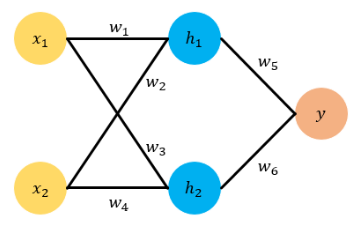
\includegraphics[scale=0.35]{HW 1 Neural Network Screenshot.png}
\end{figure}
Suppose we designed a neural network with the above structure with $x_1$ and $x_2$ as inputs and $y$ as output. $h_1$ and $h_2$ are simplified neurons without activation functions (or you can think the activation function is $y=x$). $w_1$ to $w_6$ are parameters. We have:
$$h_1 = w_1 * x_1 + w_2 * x_2$$
$$h_2 = w_3 * x_1 + w_4 * x_2$$
$$y = w_5 * h_1 + w_6 * h_2$$
We use the Backpropagation method to train this network, and let the error $E = 0.5(y-t)^2$ , where $t$ is the target (or label). If you are given the following dataset with one example:
\begin{table}[H]
    \centering
    \begin{tabular}{|c|c|c|c|}
     \hline
        Data & $x_1$ & $x_2$ & $t$ \\
     \hline
        Example 1 & 1 & 0.5 & 4 \\
     \hline
    \end{tabular}
\end{table}
and the initialized weights are: $w_1 = 0.5, w_2 = 1.5, w_3 = 2.3, w_4 = 3, w_5 = 1, w_6 = 1$
\begin{enumerate}
    \item What is the error after one epoch of feed-forward pass?\\
    $y = w_5(w_1 * x_1 + w_2 * x_2) + w_6 (w_3 * x_1 + w_4 * x_2)$\\
    $y = 1*(0.5*1+1.5*0.5)+1*(2.3*1+3*0.5) = 5.05$\\
    $E = 0.5 * (5.05-4)^2 = 0.55125$
    \item The error is not zero, so we need to update the weights following gradient descent. If we set the learning rate as $0.1$, what are the updated weights?\\
    $\gamma = 0.1$, $\frac{\partial E}{\partial y} = (y-t)$\\
    $y = w_5*h_1 + w_6*h_2 = w_5(w_1 * x_1 + w_2 * x_2) + w_6 (w_3 * x_1 + w_4 * x_2)$\\

	$\frac{\partial E}{\partial w_6}=\frac{\partial E}{\partial y} \times \frac{\partial y}{\partial w_6}=(y-t)*h_2=(y-t)*(w_3 * x_1 + w_4 * x_2)=(5.05-4)*(2.3*1+3*0.5)=3.99$\\
	$w_6 = 1 - \gamma * 3.99 = 1 - 0.1 * 3.99 = 0.601$\\
	
	$\frac{\partial E}{\partial w_5}=\frac{\partial E}{\partial y} \times \frac{\partial y}{\partial w_5}=(y-t)*h_1=(y-t)*(w_1 * x_1 + w_2 * x_2)=(5.05-4)*(0.5*1+1.5*0.5)=1.3125$\\
	$w_5=1 - \gamma * 1.3125 = 1 - 0.1 * 1.3125 = 0.86875$\\
	
	$\frac{\partial E}{\partial w_4}=\frac{\partial E}{\partial y} \times \frac{\partial y}{\partial w_4}=(y-t)*w_6 * x_2 = (5.05 - 4) * 1 * 0.5 = 0.525$\\
	$w_4=3-\gamma*0.525=3-0.1*0.525=2.9475$\\
	
	$\frac{\partial E}{\partial w_3}=\frac{\partial E}{\partial y} \times \frac{\partial y}{\partial w_3}=(y-t)*w_6*x_1 = (5.05-4)*1*1=1.05$\\
	$w_3=2.3-\gamma*1.05=2.3-0.1*1.05=2.195$\\

	$\frac{\partial E}{\partial w_2}=\frac{\partial E}{\partial y} \times \frac{\partial y}{\partial w_2}=(y-t)*w_5*x_2=(5.05-4)*1*0.5=0.525$\\
	$w_2=1.5-\gamma*0.525 = 1.5-0.1*0.525=1.4475$\\

	$\frac{\partial E}{\partial w_1}=\frac{\partial E}{\partial y} \times \frac{\partial y}{\partial w_1}=(y-t)*w_5*x_1=(5.05-4)*1*1=1.05$\\
	$w_1 = 0.5 - \gamma*1.05 = 0.5-0.1*1.05=0.395$\\
    \item With the updated weights, what is the new error? Is the error reduced?\\
    $y = w_5(w_1 * x_1 + w_2 * x_2) + w_6 (w_3 * x_1 + w_4 * x_2)$\\
	$y = 0.86875*(0.395*1+1.4475*0.5)+0.601*(2.195*1+2.9475*0.5) = 3.1768328125$\\
	$E = 0.5 * (3.1768328125 - 4)^2 = 0.33880210928$\\
	Yes, the error is reduced by 0.212447891.

\end{enumerate}

\end{document}
